\chapter{ಮೊದಲ ಪ್ರೋಗ್ರಾಂ}
ಕಂಪ್ಯೂಟರ್, ನಾವು ನೀಡುವ ಆಜ್ಞೆಗಳಂತೆ ಯಥಾವತ್ತಾಗಿ ಕೆಲಸ ಮಾಡುತ್ತದೆ.  ನಾವು ಹಿಂದಿನ ಅಧ್ಯಾಯದಲ್ಲಿ ಸ್ಕ್ರಾಚ್ ಸ್ಕ್ರೀನ್ ಅನ್ನು ನೋಡಿದೆವು. ಈಗ ನಾವು ಕೊಡುವ ಆಜ್ಞೆಗಳಿಂದಾಗಿ ಸ್ಪ್ರಯ್ಟ್  ಏನೆಲ್ಲಾ ಕೆಲಸ ಮಾಡುವುದೆಂದು ನೋಡೋಣ.  ಮೊದಲಿಗೆ "ಚಲನೆ" ಮತ್ತು "ಹಿಡಿತ" ಗುಂಪುಗಳಲ್ಲಿನ  ಆಜ್ಞೆಗಳನ್ನು ಬಳಸಿ ಸ್ಪ್ರಯ್ಟ್ ನಿಂದ ಕೆಲಸ ಮಾಡಿಸೋಣ. 



\section{ಮುಂದೆ ಹೋಗು}
\begin{figure}[h]
\begin{center}
\begin{multicols}{2}
\begin{Scratch}[1]
\beginbox{}
\scbox{\cb[w]{10} ಹೆಜ್ಜೆ ಮುಂದೆ ಹೋಗು}{motion}
\end{Scratch}

\begin{tikzpicture}
\node[doc] (x) (inst1){
ಒತ್ತಿದಾಗ\\
10  ಹೆಜ್ಜೆ ಮುಂದೆ ಹೋಗು
};
\end{tikzpicture}
\end{multicols}
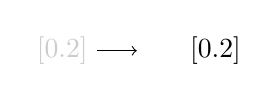
\begin{tikzpicture}
\node at (0,0)[rotate=0, opacity=0.2](s1){\Scratchy[0.2]};
\draw[->](s1.east)--++(0.5cm,0)node(newcoord){};
\node at ([shift={(1cm,0)}]newcoord)[rotate=0, opacity=1](s2){\Scratchy[0.2]};
\end{tikzpicture}
\end{center}

\caption{ಮೊದಲನೆ ಪ್ರೋಗ್ರಾಂ: ಸ್ಪ್ರಯ್ಟ್  ಅನ್ನು ಮುಂದೆ ಹೋಗಿಸುವುದು}
\label{program1}
\end{figure}

\vspace{-0.5cm}
ಮೊದಲನೆಯದಾಗಿ ಹಿಡಿತ ಗುಂಪಿನ "ಒತ್ತಿದಾಗ" ಎಂಬ ಆಜ್ಞೆಯನ್ನು ಪ್ರೊಗ್ರಾಂ ತಯಾರಿಯ ಜಾಗದಲ್ಲಿರಿಸೋಣ.  ಈ ಆಜ್ಞೆ ಏನು ಮಾಡುವುದೆಂದರೆ,  ನೀವು ಮೌಸ್ನಿಂದ ವೇದಿಕೆಯ ಮೇಲಿನ ಹಸಿರು ಧ್ವಜವನ್ನು ಒತ್ತಿದಾಗ, ಈ ಆಜ್ಞೆಯ ಕೆಳಗಿನ ಪ್ರೋಗ್ರಾಮಿನಂತೆ ಸ್ಪ್ರಯ್ಟ್ ನಿಂದ ಕೆಲಸ ಮಾಡಿಸುತ್ತದೆ. ಈಗ, "ಒತ್ತಿದಾಗ" ಆಜ್ಞೆಯ ಕೆಳಗೆ “ಹತ್ತು ಹೆಜ್ಜೆ ಮುಂದೆ ಹೋಗು” ಎಂದು ಆಜ್ಞೆಯನ್ನು ಚಲನೆ ಗುಂಪಿನಿಂದ ತಂದು ಜೋಡಿಸಿ.  ನಿಮ್ಮ ಮೊದಲನೆ ಪ್ರೋಗ್ರಾಂ ಈಗ ಚಿತ್ರ \ref{program1}  ಎಡಭಾಗದಂತೆ ಕಾಣಬೇಕು.  ಈಗ ವೇದಿಕೆಯ ಮೇಲಿನ ಹಸಿರು ಧ್ವಜವನ್ನು ಒತ್ತಿ,  ಸ್ಪ್ರಯ್ಟ್ ಹತ್ತು ಹೆಜ್ಜೆ ಮುಂದೆ ಹೋಗುವುದೇ ಪರಿಶೀಲಿಸಿ.  ಚಿತ್ರ \ref{program1}ರ ಕೆಳಭಾಗದಲ್ಲಿ ತೋರಿಸಿರುವಂತೆ ಸ್ಪ್ರಯ್ಟ್ ತಾನಿದ್ದಲ್ಲಿಂದ ಹತ್ತು ಹೆಜ್ಜೆ ಮುಂದೆ ಹೋಗಿರಬೇಕು. 

ಪ್ರೋಗ್ರಾಂಗಳನ್ನು ಸ್ಕ್ರಾಚ್ನಲ್ಲಿ ಪ್ರಯತ್ನಿಸುವ ಮುನ್ನ ಅದರಿಂದ ಏನು ಕೆಲಸ ಆಗಬೇಕು ಎನ್ನುವುದನ್ನು ಮನವರಿಕೆ ಮಾಡಿಕೊಂಡಿರಬೇಕು. ಹೀಗೆ ಮನವರಿಕೆ ಮಾಡಿಕೊಳ್ಳುವುದಕ್ಕೆ ನಾವು ಮೊದಲು ಪುಸ್ತಕದಲ್ಲಿ ಪ್ರೋಗ್ರಾಂಗಳನ್ನು ಬರೆದು ಅವು ಹೇಗೆ ಕೆಲಸ ಮಾಡಬಹುದೆಂದು ಯೋಚಿಸಬಹುದು.  ಈ ಮೊದಲನೆ ಪ್ರೋಗ್ರಾಂಗೆ ಚಿತ್ರ \ref{program1} ಬಲಭಾಗದಲ್ಲಿರುವಂತೆ ಪುಸ್ತಕದಲ್ಲಿ  ಬರೆದುಕೊಳ್ಳಬಹುದು.  ಹೀಗೆ ಅಭ್ಯಾಸ ಮಾಡುವುದರಿಂದ, ನಮಗೆ ಕಂಪ್ಯೂಟರ್ ಸಿಕ್ಕ ಬಳಿಕ ಅದನ್ನು ಉಪಯುಕ್ತ ರೀತಿಯಲ್ಲಿ ಬಳಸಬಹುದು. 

\section{ಮುಂದೆ ಹೋಗಿ ತಿರುಗು}

\begin{figure}[h]
\begin{center}
\begin{multicols}{2}
\begin{Scratch}[1]
\beginbox{}
\scbox{\cb[w]{100} ಹೆಜ್ಜೆ ಮುಂದೆ ಹೋಗು}{motion}
\turnbox{1}{90}{ಡಿಗ್ರಿಯಷ್ಟು ತಿರುಗು}
\end{Scratch}

\begin{tikzpicture}
\node[doc] (x) (inst1){
ಒತ್ತಿದಾಗ\\
100  ಹೆಜ್ಜೆ ಮುಂದೆ ಹೋಗು\\
90$‌^\circ$ ಬಲಕ್ಕೆ  ತಿರುಗು
};
\end{tikzpicture}

\end{multicols}

\begin{tikzpicture}
\node at (0,0)[rotate=0, opacity=0.2](s1){\Scratchy[0.2]};
\draw[->](s1.east)--++(2cm,0)node(newcoord){};
\node at ([shift={(1cm,0)}]newcoord)[rotate=-90, opacity=1](s2){\Scratchy[0.2]};
\end{tikzpicture}
\end{center}
\caption{ಸ್ಪ್ರಯ್ಟ್ ಮುಂದೆ ಹೋದ ಮೇಲೆ ಬೇಕಾದಂತೆ ತಿರುಗಿಸುವುದು}
\label{program2}
\end{figure}

ಸ್ಪ್ರಯ್ಟ್ ಮುಂದೆ ಹೋದ ಮೇಲೆ ನಮಗೆ ಬೇಕಾದಂತೆ ತಿರುಗಿಸುವುದು ಹೇಗೆ ಎಂದು ನೋಡೋಣ. ಮೊದಲಿನಂತೆ, ಹಿಡಿತ ಗುಂಪಿನ "ಒತ್ತಿದಾಗ" ಎಂಬ ಆಜ್ಞೆಯನ್ನು ಪ್ರೊಗ್ರಾಂ ತಯಾರಿಯ ಜಾಗದಲ್ಲಿರಿಸಿ, ಅದಕ್ಕೆ “ಹತ್ತು ಹೆಜ್ಜೆ ಮುಂದೆ ಹೋಗು” ಎಂಬ ಆಜ್ಞೆಯನ್ನು ಚಲನೆ ಗುಂಪಿನಿಂದ ತಂದು ಜೋಡಿಸಿ.  ಈ ಆಜ್ಞೆಯಲ್ಲಿ 10 ಸಂಖ್ಯೆಯನ್ನು 100 ಕ್ಕೆ ಬದಲಾಯಿಸಿ.  ಇವೆರಡರ ಕೆಳಗೆ,  "90 ಡಿಗ್ರಿಯಷ್ಟು ತಿರುಗು" ಎಂಬ ಆಜ್ಞೆಯನ್ನು ತಂದು ಜೋಡಿಸಿ.  ಈ ಆಜ್ಞೆಯಲ್ಲಿ ತಿರುಗುವ ದಿಕ್ಕು ಯವುದಿದೆ ಎಂದು ಪರೀಕ್ಷಿಸಿಕೊಳ್ಳಿ. ನಿಮ್ಮ ಪ್ರೋಗ್ರಾಂ ಈಗ ಚಿತ್ರ \ref{program2}  ಎಡಭಾಗದಂತೆ ಕಾಣಬೇಕು.    ವೇದಿಕೆಯ ಮೇಲಿನ ಹಸಿರು ಧ್ವಜವನ್ನು ಒತ್ತಿ,  ಸ್ಪ್ರಯ್ಟ್ ನೂರು ಹೆಜ್ಜೆ ಮುಂದೆ ಹೋಗಿ, ಬಲಕ್ಕೆ ತಿರುಗುವುದೇ, ಪರಿಶೀಲಿಸಿ.  ಚಿತ್ರ \ref{program2}ರ ಕೆಳಭಾಗದಲ್ಲಿ ತೋರಿಸಿರುವಂತೆ ಸ್ಪ್ರಯ್ಟ್ ತಾನಿದ್ದಲ್ಲಿಂದ ನೂರು ಹೆಜ್ಜೆ ಮುಂದೆ ಹೋಗಿ ಬಲಕ್ಕೆ 90 ಡಿಗ್ರಿ ತಿರುಗಿರಬೇಕು.  ಚಿತ್ರ \ref{program2}ನ ಬಲಭಾಗದಲ್ಲಿರುವಂತೆ  ಅಭ್ಯಾಸಕ್ಕಾಗಿ ಪುಸ್ತಕದಲ್ಲಿ  ಪ್ರೋಗ್ರಾಂ ಅನ್ನು ಸರಳವಾಗಿ ಬರೆದುಕೊಳ್ಳಬಹುದು. 

ಈಗ ಕಲಿತಿರುವ ಆಜ್ಞೆಗಳನ್ನೇ ಉಪಯೋಗಿಸಿಕೊಂಡು ಒಂದು ಕುತೂಹಲಕಾರಿ ಪ್ರೋಗ್ರಾಂ ಅನ್ನು ರಚಿಸೋಣ.  ಈಗ ಚಿತ್ರ \ref{program3}  ಎಡಭಾಗದಂತೆ ಆಜ್ಞೆಗಳನ್ನು ತಂದು ಜೋಡಿಸಿ.    

\begin{figure}[h]
\begin{center}
\begin{multicols}{2}
\begin{Scratch}[1]
\beginbox{}
\scbox{\cb[w]{100} ಹೆಜ್ಜೆ ಮುಂದೆ ಹೋಗು}{motion}
\turnbox{1}{90}{ಡಿಗ್ರಿಯಷ್ಟು ತಿರುಗು}
\scbox{\cb[w]{100} ಹೆಜ್ಜೆ ಮುಂದೆ ಹೋಗು}{motion}
\turnbox{1}{90}{ಡಿಗ್ರಿಯಷ್ಟು ತಿರುಗು}
\scbox{\cb[w]{100} ಹೆಜ್ಜೆ ಮುಂದೆ ಹೋಗು}{motion}
\turnbox{1}{90}{ಡಿಗ್ರಿಯಷ್ಟು ತಿರುಗು}
\scbox{\cb[w]{100} ಹೆಜ್ಜೆ ಮುಂದೆ ಹೋಗು}{motion}
\end{Scratch}

\begin{tikzpicture}
\node[doc] (x) (inst1){
ಒತ್ತಿದಾಗ\\
100  ಹೆಜ್ಜೆ ಮುಂದೆ ಹೋಗು\\
90$‌^\circ$ ಬಲಕ್ಕೆ  ತಿರುಗು\\
100  ಹೆಜ್ಜೆ ಮುಂದೆ ಹೋಗು\\
90$‌^\circ$ ಬಲಕ್ಕೆ  ತಿರುಗು\\
100  ಹೆಜ್ಜೆ ಮುಂದೆ ಹೋಗು\\
90$‌^\circ$ ಬಲಕ್ಕೆ  ತಿರುಗು\\
100  ಹೆಜ್ಜೆ ಮುಂದೆ ಹೋಗು
};
\end{tikzpicture}

\end{multicols}

\begin{tikzpicture}
\node at (0,0)[rotate=0, opacity=0.2](s1){\Scratchy[0.2]};
\draw[->](s1.east)--++(2cm,0)node(newcoord){};
\node at ([shift={(1cm,0)}]newcoord)[rotate=-90, opacity=0.2](s2){\Scratchy[0.2]};
\draw[->](s2.east)--++(0,-2cm)node(newcoord){};
\node at ([shift={(0,-1cm)}]newcoord)[rotate=-180, opacity=0.2](s3){\Scratchy[0.2]};
\draw[->](s3.east)--++(-2cm,0cm)node(newcoord){};
\node at ([shift={(-1cm,0)}]newcoord)[rotate=90, opacity=0.2](s4){\Scratchy[0.2]};
\draw[->](s4.east)--++(0,2cm)node(newcoord){};
\node at ([shift={(0,1cm)}]newcoord)[rotate=90, opacity=1](s2){\Scratchy[0.2]};
\end{tikzpicture}
\end{center}
\caption{ಸ್ಪ್ರಯ್ಟ್ ಅನ್ನು ಚೌಕಾಕಾರವಾಗಿ ಚಲಾಯಿಸುವುದು}
\label{program3}
\end{figure}

ನಿಮ್ಮ ಪ್ರೋಗ್ರಾಂ ಈಗ ಚಿತ್ರ \ref{program3}  ಎಡಭಾಗದಂತೆ ಕಾಣಬೇಕು.   ಪ್ರೋಗ್ರಾಂ ಅನ್ನು  ಚಲಾಯಿಸಿ (ವೇದಿಕೆಯ ಮೇಲಿನ ಹಸಿರು ಧ್ವಜವನ್ನು ಒತ್ತಿ),  ಸ್ಪ್ರಯ್ಟ್ ಮುಂದೆ ಹೋಗಿ, ಬಲಕ್ಕೆ ತಿರುಗುವುದನ್ನು ನಾಲ್ಕು ಬಾರಿ ಮಾಡುವುದೇ ಎಂದು ಪರಿಶೀಲಿಸಿ.  ಚಿತ್ರ \ref{program3}ರ ಕೆಳಭಾಗದಲ್ಲಿ ತೋರಿಸಿರುವಂತೆ ಸ್ಪ್ರಯ್ಟ್ ತಾನಿದ್ದಲ್ಲಿಂದ ನೂರು ಹೆಜ್ಜೆ ಮುಂದೆ ಹೋಗಿ ಬಲಕ್ಕೆ 90 ಡಿಗ್ರಿ ನಾಲ್ಕು ಬಾರಿ ತಿರುಗಿರಬೇಕು.  ಸ್ಪ್ರಯ್ಟ್ ಹೀಗೆ ಹಂತ ಹಂತವಾಗಿ ಕೆಲಸ ಮಾಡುವುದು ನಮ್ಮ ಕಣ್ಣಿಗೆ ಕಾಣುತ್ತದೆಯೇ? ಏಕೆ ಕಾಣುವುದಿಲ್ಲ ಎಂದು ಒಮ್ಮೆ ಯೋಚಿಸಿ. 

ಚಿತ್ರ \ref{program3}ನ ಬಲಭಾಗದಲ್ಲಿರುವಂತೆ  ಈ ಪ್ರೊಗ್ರಾಂ ಆನ್ನು ಪುಸ್ತಕದಲ್ಲಿ  ಸರಳವಾಗಿ ಬರೆದುಕೊಳ್ಳಬಹುದು.   ಇದರಲ್ಲಿ ಗಮನಿಸಿ, ಸ್ಪ್ರಯ್ಟ್  ತಾನು ಮೊದಲಿದ್ದ ದಿಕ್ಕಿನಲ್ಲಿ ಮುಖ ಮಾಡಿ ನಿಂತಿಲ್ಲ. ಏಕೆ? ಅದು ಮೊದಲಿದ್ದ ದಿಕ್ಕಿನಲ್ಲಿ ಮುಖ ಮಾಡಿ ನಿಲ್ಲಬೇಕಾದರೆ ಪ್ರೋಗ್ರಾಂ ಅನ್ನು ಹೇಗೆ ಬದಲಾಯಿಸ ಬೇಕು? ಈ ಸವಾಲು  ಒದುಗರ ಪ್ರಯತ್ನಕ್ಕೆ.

\section{ಕಾಯುವುದು}
ಕಂಪ್ಯೂಟರ್, ನಾವು ನೀಡುವ ಆಜ್ಞೆಗಳಂತೆ ಯಥಾವತ್ತಾಗಿ ಅತಿವೇಗವಾಗಿ ಕೆಲಸ ಮಾಡಿಬಿಡುತ್ತದೆ. ಹಾಗಾಗಿ ಅದು ಹಂತ ಹಂತವಾಗಿ ಕೆಲಸ ಮಾಡುವುದು ನಮ್ಮ ಕಣ್ಣಿಗೆ ಕಾಣುವುದಿಲ್ಲ.  ನಮಗೆ ಕಾಣಿಸಬೇಕಾದರೆ,  ಪ್ರೊಗ್ರಾಂ ಆನ್ನು ನಮಗೆ ಬೇಕಾದ ಹಂತಗಳಲ್ಲಿ ತಡೆದು ಕಾಯಿಸಬೇಕು - ಹೇಗೆ ಎಂದು ಈಗ ನೋಡೋಣ.


\begin{figure}[h]
\begin{center}
\begin{multicols}{2}
\begin{Scratch}[1]
\beginbox{}
\scbox{\cb[w]{100} ಹೆಜ್ಜೆ ಮುಂದೆ ಹೋಗು}{motion}
\scbox{\cb[w]{1}  ಸೆಕೆಂಡುಗಳಷ್ಟು   ಕಾಯಬೇಕು}{control}
\turnbox{1}{90}{ಡಿಗ್ರಿಯಷ್ಟು ತಿರುಗು}
\scbox{\cb[w]{1}  ಸೆಕೆಂಡುಗಳಷ್ಟು   ಕಾಯಬೇಕು}{control}
\scbox{\cb[w]{100} ಹೆಜ್ಜೆ ಮುಂದೆ ಹೋಗು}{motion}
\scbox{\cb[w]{1}  ಸೆಕೆಂಡುಗಳಷ್ಟು   ಕಾಯಬೇಕು}{control}
\turnbox{1}{90}{ಡಿಗ್ರಿಯಷ್ಟು ತಿರುಗು}
\scbox{\cb[w]{1}  ಸೆಕೆಂಡುಗಳಷ್ಟು   ಕಾಯಬೇಕು}{control}
\scbox{\cb[w]{100} ಹೆಜ್ಜೆ ಮುಂದೆ ಹೋಗು}{motion}
\scbox{\cb[w]{1}  ಸೆಕೆಂಡುಗಳಷ್ಟು   ಕಾಯಬೇಕು}{control}
\turnbox{1}{90}{ಡಿಗ್ರಿಯಷ್ಟು ತಿರುಗು}
\scbox{\cb[w]{1}  ಸೆಕೆಂಡುಗಳಷ್ಟು   ಕಾಯಬೇಕು}{control}
\scbox{\cb[w]{100} ಹೆಜ್ಜೆ ಮುಂದೆ ಹೋಗು}{motion}
\scbox{\cb[w]{1}  ಸೆಕೆಂಡುಗಳಷ್ಟು   ಕಾಯಬೇಕು}{control}
\turnbox{1}{90}{ಡಿಗ್ರಿಯಷ್ಟು ತಿರುಗು}
\end{Scratch}

\begin{tikzpicture}
\node[doc] (x) (inst1){
ಒತ್ತಿದಾಗ\\
100  ಹೆಜ್ಜೆ ಮುಂದೆ ಹೋಗು\\
1 ಸೆಕೆಂಡುಗಳಷ್ಟು   ಕಾಯಬೇಕು\\
90$‌^\circ$ ಬಲಕ್ಕೆ  ತಿರುಗು\\
1 ಸೆಕೆಂಡುಗಳಷ್ಟು   ಕಾಯಬೇಕು\\
100  ಹೆಜ್ಜೆ ಮುಂದೆ ಹೋಗು\\
1 ಸೆಕೆಂಡುಗಳಷ್ಟು   ಕಾಯಬೇಕು\\
90$‌^\circ$ ಬಲಕ್ಕೆ  ತಿರುಗು\\
1 ಸೆಕೆಂಡುಗಳಷ್ಟು   ಕಾಯಬೇಕು\\
100  ಹೆಜ್ಜೆ ಮುಂದೆ ಹೋಗು\\
1 ಸೆಕೆಂಡುಗಳಷ್ಟು   ಕಾಯಬೇಕು\\
90$‌^\circ$ ಬಲಕ್ಕೆ  ತಿರುಗು\\
1 ಸೆಕೆಂಡುಗಳಷ್ಟು   ಕಾಯಬೇಕು\\
100  ಹೆಜ್ಜೆ ಮುಂದೆ ಹೋಗು\\
1 ಸೆಕೆಂಡುಗಳಷ್ಟು   ಕಾಯಬೇಕು\\
90$‌^\circ$ ಬಲಕ್ಕೆ  ತಿರುಗು
};
\end{tikzpicture}
\end{multicols}
\end{center}
\caption{ಸ್ಪ್ರಯ್ಟ್ ಆನು ಹಂತ ಹಂತವಾಗಿ ಕಾಯ್ದಿರಿಸಿ ಪ್ರೊಗ್ರಾಮ್ಮನ್ನು ವಿಶ್ಲೇಷಿಸುವುದು}
\label{program3}
\end{figure}


\section{ಅಭ್ಯಾಸ }

\begin{center}
\begin{figure}
\begin{multicols}{2}
\begin{Scratch}[1]
\scbox{\cb[w]{10}  ಹೆಜ್ಜೆ ಮುಂದೆ ಹೋಗು}{motion}
\scbox{\cb[w]{20}  ಹೆಜ್ಜೆ ಮುಂದೆ ಹೋಗು}{motion}
\end{Scratch}


\begin{tikzpicture}
\node[doc] (x) (inst1){
10  ಹೆಜ್ಜೆ ಮುಂದೆ ಹೋಗು\\
20  ಹೆಜ್ಜೆ ಮುಂದೆ ಹೋಗು
};
\end{tikzpicture}
\end{multicols}

\caption{}
\label{writing}
\end{figure}
\end{center}


\begin{center}
\begin{figure}
\begin{multicols}{2}
\begin{Scratch}[1]
\boucle{\cb[w]{4} ಮರುಕಳಿಸು}{1}{1}
\scbox{\cb[w]{20}  ಹೆಜ್ಜೆ ಮುಂದೆ ಹೋಗು}{motion}
\scbox{\cb[w]{50}  ಹೆಜ್ಜೆ ಮುಂದೆ ಹೋಗು}{motion}
\end{Scratch}


\begin{tikzpicture}
\node[doc] (x) (inst1){
4 ಮರುಕಳಿಸು\\
\hspace{0.6cm}20  ಹೆಜ್ಜೆ ಮುಂದೆ ಹೋಗು\\
50  ಹೆಜ್ಜೆ ಮುಂದೆ ಹೋಗು
};
\end{tikzpicture}
\end{multicols}

\caption{}
\label{writing}
\end{figure}
\end{center}
